\documentclass[12pt,a4paper]{article}
\usepackage[utf8]{inputenc}
\usepackage[portuguese]{babel}
\usepackage[T1]{fontenc}
\usepackage{amsfonts, amssymb, amsmath, dsfont}	% fonte e simbolos matemáticos
\usepackage{graphicx}
\usepackage{type1ec} 
\usepackage[left=3cm,right=3cm,top=3cm,bottom=3cm]{geometry}

%% Tabelas com melhor espaçamento
\renewcommand{\arraystretch}{1.5}
\setlength\tabcolsep{5pt}



\author{Raquel}
\title{Resultados Gráficos do TCC}
\begin{document}

\section{Testes de Estabilidade}

O gráfico mostra os tempos obtidos em 10 execuções, sendo cada uma com um conjunto de dados diferente. 
O tempo do quicksort foi menor em todas as execuções, mas a diferença é bem pequena. 
A variação dos tempos também é pequena, a variação entre o maior e menor tempo foi de menos de 2 segundos. A tabela mostra as
estatísticas para o teste. 

\begin{table}[!htb]
\begin{tabular}{|c|c|c|c|c|c|c|c|} \hline
Algoritmo & Menor & Maior & Média & Mediana & Variância & Desvio Padrão & COV \\
\hline 
Quicksort & 18.449  & 20.086  & 18.7865  & 18.4895  & 0.294432  & 0.542616  & 0.0288833 \\ 
\hline 
Samplesort & 19.44  & 20.622 & 19.8422 & 19.482 & 0.250538 & 0.500538 &  0.025226 \\ 
\hline 
\end{tabular}%\caption{•}
\end{table}


Fiz um gráfico igual ao feito no trabalho da Paula contendo os tempos dos dois algoritmos. 
\begin{figure}[!htb]
\centering
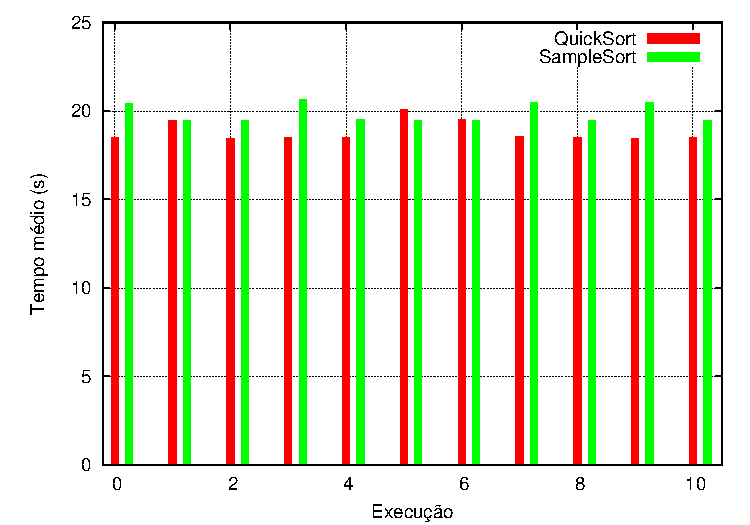
\includegraphics{Estabilidade/EstabilidadeTempo.pdf} 
\caption{Tempo (s): Teste de Estabilidade}
\end{figure}

\newpage

\section{Testes variando o número de partições}


Esse teste foi o sugerido naquele email, para variar o número de partições
para menos e manter o número de máquinas constante. 
As partições foram 8, 6, 4 e 2, e o tempo diminui consideravelmente com menos partições. 
(O gráfico mostra de forma crescente o número de partições, mas pensei que se for mostrado de maneira decrescente vai ser mais interessante.)


O esperado para o sample sort era o contrário, quanto maior o número de partições, melhor o desempenho, e de fato isso ocorre, mas de maneira menos acentuada. (Fiz o teste com o sample sort mais para ver como seria, talvez nem seja preciso incluir nos resultados.)

Esse teste é interessante porque justifica o uso de duas partições nos demais testes. Como foi verificado que o melhor tempo é com 2 partições, passei a utilizar esse valor para partições. \\
 
\begin{figure}[!htb]
\includegraphics{Particoes/VariandoParticoesTempo.pdf} 
\caption{Tempo(s): ordenação de $10^8$ dados com diferente número de partições}
\end{figure}

A Figura 3 é o coeficiente de variação das partições, que mostra uma variação um pouco maior com o Quicksort. 
\begin{figure}[!htb]
\includegraphics{Particoes/VariandoParticoesParticoes.pdf} 
\caption{COV das partições}
\end{figure}


\newpage

\section{Testes variando os dados de $10^6$ a $10^{10}$}

Esse teste foi variando a quantidade de dados, com um número constante de máquinas.
Você havia comentado na reunião sobre a quantidade de dados ser 4, e continuávamos com essa quantidade porque
já haviam testes executados nesse número. Como a manutenção na rede deu muita alteração no tempo,
eu refiz os testes com os dois algoritmos usando as 5 máquinas disponíveis. 

Para o quicksort foi executado com 2 partições, e para o sample sort mantive a fórmula anteriormente usada:
partições = máquinas x núcleos. 

O tempo do quicksort foi ligeiramente menor com $10^6$ e  maior nos demais casos. Quanto maior o arquivo, maior a diferença entre os tempos. 
Para cada tamanho de arquivo, executei 5 testes, e o gráfico inclui a média dos tempos para as 5 execuções. Ainda é preciso incluir os dados das execuções de $10^{10}$.

\begin{figure}[!htb]
\includegraphics{Dados/VariandoDadosTempo.pdf} 
\caption{Tempo (s): Teste variando dados de $10^6$ a $10^{10}$}
\end{figure}

Fiz também um gráfico incluindo o tempo para ordenação de cada $10^6$ dados (MegaDados). 
\begin{figure}[!htb]
\includegraphics{Dados/VariandoDadoMegaDados.pdf} 
\caption{Tempo (s): avaliando a ordenação de MegaDados (arquivos de $10^6$ a $10^{10}$) }
\end{figure}


\newpage

\section{Testes variando o número de máquinas}

Os testes variando o número de máquinas são os mais interessantes para o sample sort, porque mostram o speed up e a eficiência.
Para o quicksort também há uma melhora considerável no tempo, mesmo sendo o número constante de 2 partições. 

Os gráficos de speed up e eficiência ainda não estão prontos, assim que estiverem eu enviarei. 

\begin{figure}[!htb]
\includegraphics{Maquinas/VariandoMaquinasTempo.pdf} 
\caption{Tempo (s): ordenação de $10^8$ dados em número variável de máquinas}
\end{figure}


\newpage


\section{Testes variando a distribuição}

Pensei em uma nova maneira para exibir os dados de distribuição.
Considerando que a variação é bastante pequena no tempo, talvez possamos criar uma nova seção para testes com distribuições diferentes, 
e não incluir o resultado de cada distribuição em todos os testes. 
Ainda não pensei exatamente como seria isso, mas fiz um gráfico de uma possível maneira, incluindo o tempo médio das três distribuições com os dois algoritmos.
Esse gráfico mostra o tempo médio de 10 execuções de $10^6$ em 5 máquinas. 

\begin{figure}[!htb]
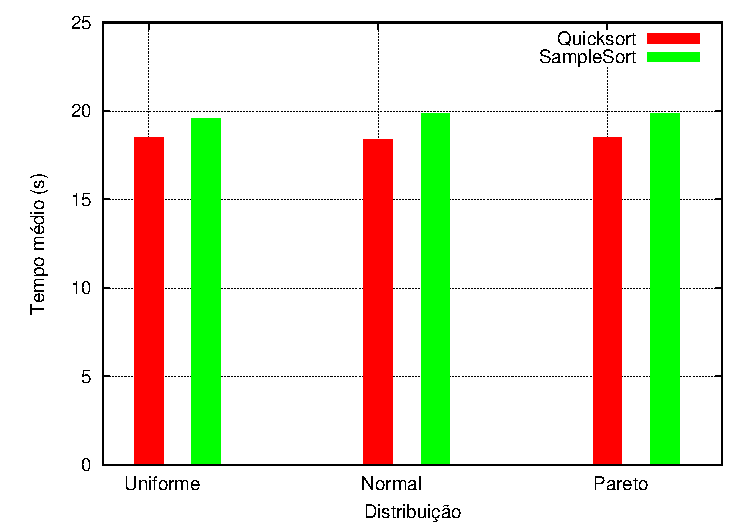
\includegraphics{Distribuicao/VariandoDistribuicaoTempo.pdf} 
\caption{Tempo(s): ordenação de $10^6$ dados das três distribuições }
\end{figure}

Essa figura é para exibir o COV das partições, que varia entre as 3 distribuições, mas influência pouco no tempo geral de ordenação.
\begin{figure}[!htb]
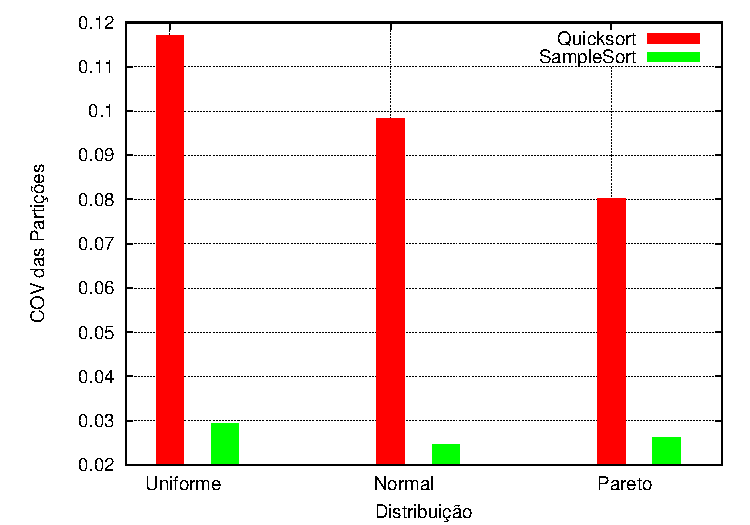
\includegraphics{Distribuicao/VariandoDistribuicaoParticoes.pdf} 
\caption{COV das partições nas três distribuições }
\end{figure}

\end{document}